\chapter{Overview}

\section{Introduction}
Forecasting time series data is a critical task in various domains, including finance, retail, healthcare, and manufacturing. It involves predicting future values based on previously observed data, and selecting the right model or algorithm for the task can greatly impact the accuracy and reliability of predictions. The goal of this project is to explore and evaluate a range of forecasting algorithms available in Python, analyzing their strengths and weaknesses through hands-on experimentation with a benchmark dataset.

This project aims to provide a broad yet practical understanding of various forecasting techniques and the Python packages that implement them. Specifically, we will experiment with the following algorithms:

\begin{enumerate}
	\item \textbf{Gaussian Processes (via PyMC):} A non-parametric Bayesian approach to modeling time series data that can provide uncertainty estimates along with predictions.
	\item \textbf{Bayesian Two-layer Perceptron (via PyMC and TensorFlow/Keras):} A neural network model with a Bayesian framework to quantify uncertainty in the predictions.
	\item \textbf{Kalman Filter (via filterpy):} A recursive algorithm for linear dynamic systems that estimates the state of a process in real-time.
	\item \textbf{Decision Trees (via XGBoost, LightGBM, PyMC):} A non-linear, non-parametric approach that uses ensembles of decision trees for regression tasks.
	\item \textbf{Prophet (via Prophet):} A decomposable time series model designed for forecasting at scale with an emphasis on interpretability.
	\item \textbf{LSTM (via TensorFlow/Keras):} A type of recurrent neural network that is well-suited for modeling sequential data with long-term dependencies.
	\item \textbf{SARIMAX (via statsmodels):} An extension of the ARIMA model that includes seasonality, exogenous regressors, and error correction mechanisms.
	\item \textbf{Exponential Smoothing (via statsmodels):} A method for forecasting univariate time series by weighting past observations exponentially.
	\item \textbf{Sorcerer (via PyMC):} A Prophet-inspired Generalized Additive Model (GAM) implemented in PyMC, which combines the flexibility of GAMs with Bayesian modeling techniques to provide robust time series forecasts.
\end{enumerate}

For each method, we will utilize appropriate Python packages, such as PyMC for Bayesian methods, TensorFlow/Keras for deep learning models, and statsmodels for traditional statistical models. The project will be managed using Visual Studio Code with Anaconda, and version control will be handled with Git, creating a repository for each competency development project.


\section{Data}
To benchmark the forecasting algorithms, we will use the M5 dataset, a widely recognized dataset in the forecasting community. The M5 dataset contains daily sales data from Walmart's stores and departments across various geographical locations in the United States. This dataset is available from the \href{https://www.kaggle.com/competitions/m5-forecasting-accuracy/}{M5 Forecasting Competition on Kaggle} and provides a comprehensive and challenging setting to test a broad range of forecasting algorithms due to its scale, granularity, and multiple hierarchies (e.g., store, department, and product categories).



We will focus on the weekly aggregated sales data for a particular store-category combination, specifically household sales. The time range of interest spans from 2011 to 2016. For this analysis, the data before 2012 and after 2015 is discarded. The initial period is removed to eliminate potential startup effects and noise from the early data collection phase, while the final period is excluded to simplify the evaluation by using complete calendar years. 

\begin{figure}[h]
	\centering
	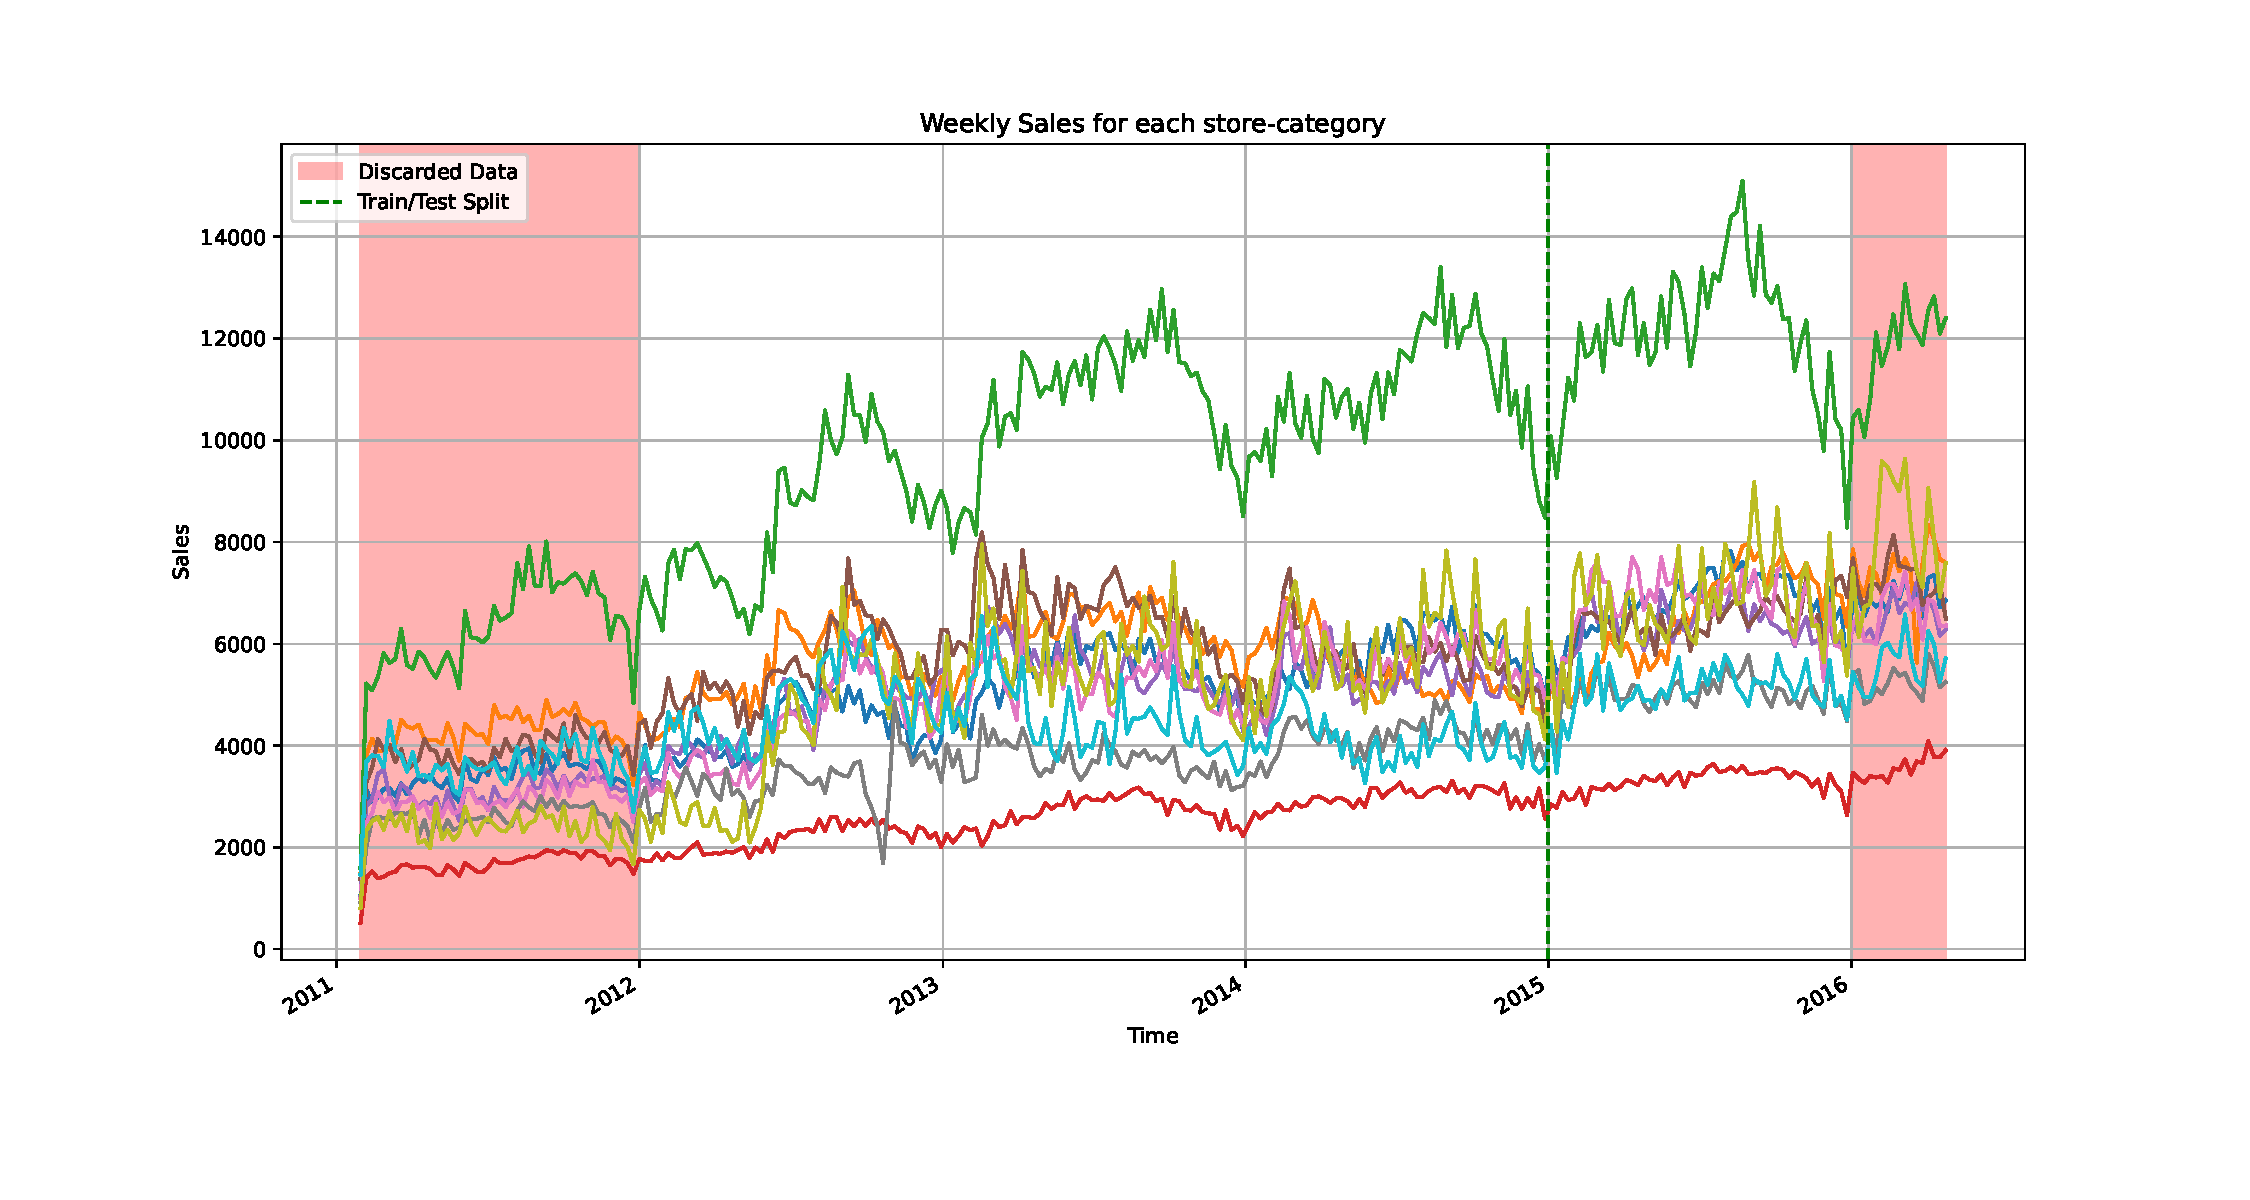
\includegraphics[width=1\textwidth]{./figures/raw_data.pdf}
	\caption{Weekly Sales for Each Store-Category}
	\label{fig:weekly_sales}
\end{figure}

The remaining data is then split into training and testing sets based on a specified date (`2015-01-01`), ensuring the training data ends with a full calendar year, accommodating a "profile" approach to forecasting. This approach facilitates the models in capturing seasonal patterns and other calendar-based trends more effectively.

Figure \ref{fig:weekly_sales} visualizes the aggregated weekly sales data after discarding the initial and final periods. The highlighted areas represent the discarded data, and the dashed vertical line indicates the split point between the training and test sets. This visualization helps to understand the overall sales trend and the data points to be retained for model training and evaluation.

The dataset and its visualization serve as the basis for comparing different forecasting methods, highlighting their capabilities in capturing patterns and making accurate predictions.

\section{Metric}